\documentclass[10pt,a4paper]{article}
\usepackage[utf8]{inputenc}
\usepackage[italian]{varioref}
\usepackage{amsmath}
\usepackage{amsfonts}
\usepackage{amssymb}
\usepackage{graphicx}
\usepackage{hyperref}
\begin{document}
\tableofcontents
\newpage
%///////////////////////////////////////////////////////////////
%   capitolo 1
%///////////////////////////////////////////////////////////////
\section{Concetti Fondamentali}
\subsection{Programma sequenziale}
Un programma sequenziale è tipicamente deterministico; ciò significa che date le stesse condizioni, gli stessi input, esso seguirà lo stesso percorso/flusso/thread di esecuzione, producendo lo stesso risultato. Esso ha un singolo thread di controllo.

\subsection{Programma concorrente o parallelo}
Due o più processi, o entità di esecuzione separate che cooperano, per ottenere un risultato.
Un CP ha più flussi di esecuzioni, quindi più thread di controllo.
Tipicamente un CP è non deterministico, e la comunicazione tra le varie entità che costituiscono il CP avviene o mediante \textbf{variabili condivise (memoria condivisa)} o mediante \textbf{scambio di messaggi}, modello utilizzato quando non c'è area di memoria comune.
Per far funzionare il tutto e per imporre dei vincoli che garantiscono la corretta esecuzione del CP (e.g. to ensure that the producer and consumer do not access the buffer at the same time, and hence that a partially written message is not read prematurely.) occorre la \textbf{sincronizzazione}.
La sincronizzazione è composta dalla \textbf{mutua esclusione}, ovvero il sistema che impedisce l'accesso alla stessa area di memoria o allo stesso set di istruzioni di sezione critica , e dalla \textbf{sincronizzazione su condizione}, che impone dei vincoli temporali, ovvero ritarda l'esecuzione di un processo finché una data condizione è vera.
(e.g. to ensure that a message is not read by the consumer until after it has been written by the producer.)

\subsection{History}
La programmazione concorrente è nata negli anni '60 nel contesto dei sistemi operativi. La motivazione era l'invenzione di unità hardware chiamate canali o controllori di dispositivi. Queste operano indipendentemente da un processore di controllo e permettono l'esecuzione di un'operazione di I/O in concomitanza con la continua esecuzione di istruzioni di programma da parte del processore centrale.
La sfida della programmazione che risultò dall'introduzione dei canali era che ora le parti di un programma potevano essere eseguite in un ordine imprevedibile. Quindi, se una parte di un programma sta aggiornando il valore di una variabile, potrebbe verificarsi un interrupt e portare ad un'altra parte del programma che cerca di cambiare il valore della stessa variabile. Questo problema specifico è conosciuto come il problema della sezione critica.

\subsection{Scrivere un CP}
Quando si scrive un programma concorrente si devono prendere decisioni su quali tipi di processi impiegare, quanti usarne e come dovrebbero interagire. Queste decisioni sono influenzate dall'applicazione, dall'hardware su cui il programma verrà eseguito e dal sistema operativo. Un programma sequenziale non a questi problemi, sostanzialmente è universale. Quindi il CP va scritto \textbf{ad hoc} per la macchina che lo eseguirà.
Qualunque siano le scelte fatte, la \textbf{chiave} per sviluppare un programma corretto è assicurare che l'interazione tra i processi sia adeguatamente \textbf{sincronizzata}. Tutto ciò per ottenere una soluzione ottimale in quanto a correttezza di risultato e prestazioni.
Esiste un compilatore parallelizzante che rende un programma automaticamente parallelo? Sacro Graal, non esiste una soluzione precisa => Serve intuito, fantasia, prove, esperimenti, cose che non si possono "donare" a un software (non ancora(?)). Quindi in generale non esiste un software che svolge questa funzione e ciò resta in carico all'ingegno umano.

\paragraph{Programmi imperativi}
classici programmi che scriviamo tutt'ora, in cui dichiaro variabili, statements e condizioni, e in cui bisogna programmare esplicitamente la concorrenza quindi usare delle primitive per far comunicare e sincronizzare i vari processi che vengono eseguiti.

\paragraph{Programmi dichiarativi, funzionali}
in cui la concorrenza è implicita e non c'è lettura e scrittura dello stato del programma. Nei programmi dichiarativi, parti indipendenti del programma possono essere eseguite in parallelo; comunicano e si sincronizzano implicitamente quando una parte dipende dai risultati prodotti da un'altra. (linguaggio PROLOG)

Su un processore singolo a time sharing ogni processo viene eseguito alla propria velocità. Non è detto che un programma di 30 righe di codice impieghi meno tempo di esecuzione di un programma da 10000 righe. Questo per motivi di scheduling

MIMD macchine che su processori separati eseguono programmi e processi propri che non hanno dati in comune. Questi possono comunicare tramite memoria condivisa o memoria distribuita.
Questa classe di macchine include multiprocessori a memoria condivisa multiprocessori, multicomputer a memoria distribuita e reti di workstation.

\subsection{Shared-memory Multiprocessors}
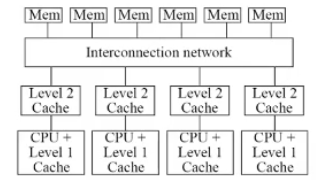
\includegraphics[scale=1]{img/sharedmem.png} \\
In un multiprocessore a memoria condivisa, i processori e i moduli di memoria sono collegati per mezzo di una rete di interconnessione. I processori condividono la memoria primaria, ma ogni processore ha la propria cache.
In base al numero di processori che compongono la macchina e alla rete di interconnessione che li collega si distinguono macchine \textbf{UMA e NUMA}.
\subsubsection{UMA} Macchina multiprocessore in cui tutti i processori hanno tempo di accesso uniforme ad ogni locazione di memoria.
Macchine composte da poche decine di processori.
\subsubsection{NUMA} Macchina con centinaia di processori che hanno una memoria organizzata gerarchicamente. In particolare, la rete di interconnessione è un insieme strutturato ad albero di switch e memorie. Di conseguenza ogni processore ha locazioni di memoria più vicine rispetto ad altre. Su questi sistemi il livello di configurazione ed ottimizzazione si fa più avanzato perché per avere buone prestazioni bisogna che un processore utilizzi una memoria quanto più vicina ad esso.

Su entrambe le macchine UMA e NUMA, ogni processore ha la propria cache. Se due processori fanno riferimento a diverse posizioni di memoria, il contenuto di queste posizioni possono tranquillamente trovarsi nelle cache dei due processori. Tuttavia, i problemi possono sorgere quando due processori fanno riferimento alla stessa locazione di memoria più o meno nello stesso momento.
Se entrambi i processori leggono la stessa posizione, ognuno può caricare una copia dei dati nella sua cache locale. Ma se un processore scrive nella posizione, c'è un \textbf{problema di coerenza della cache}: la cache dell'altro processore non contiene il valore corretto. Quindi, o l'altra cache deve essere aggiornata con il nuovo valore o la voce della cache deve essere invalidata. Soluzione al problema: ogni multiprocessore
deve implementare un protocollo di coerenza della cache nell'hardware.
Ci sono differenti modelli di consistenza della memoria:
\begin{itemize}
\item Consistenza sequenziale (strongest): garantisce che gli aggiornamenti della memoria avvengano in un qualche ordine sequenziale, e che ogni processore vedrà lo stesso ordine. \`{E} complicata da realizzare e penalizza fortemente le prestazioni.
\item Coerenza del processore: assicura che le scritture di ogni processore avvengano in memoria
nell'ordine in cui sono state emesse dal processore, ma le scritture emesse da diversi 
processori potrebbero essere viste in ordini diversi dagli altri processori.
\item Rilascio è un modello ancora più debole; assicura solo che la memoria primaria sia aggiornata ai punti di sincronizzazione specificati dal programmatore.
\end{itemize}

\subsection{Sistemi a memoria distribuita}
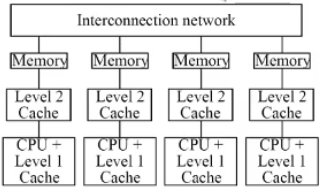
\includegraphics[scale=1]{img/distrmem.png} \\
In un multiprocessore a memoria distribuita, c'è di nuovo una rete di interconnessione, ma ogni processore ha la sua memoria privata. Sistema che si presta ad ospitare programmi che funzionano mediante message passing. Questo schema può essere utilizzato a vari livelli di coesione: 
\begin{itemize}
\item multicomputer: tightly coupled machine (macchina a coesione stretta) in cui processori e rete sono molto vicini tra loro, si trovano nello stesso armadio. Garantisce comunicazione ad alta velocità tra i processori.
\item network computer: loosely coupled, multiporcessori connessi tramite rete locale o internet. Velocità di comuinicazione minore rispetto all'altro schema in favore di una comodità di assemblaggio della working station.
\end{itemize}

\subsection{Application and Programming Styles}
Ci sono tre ampie classi di applicazioni della programmazione concorrente: sistemi multithreaded, sistemi distribuiti e computazioni parallele.
\paragraph{Multithreaded apps} Essenzialmente significa più processi che processori, tipicamente più processi e un processore che viene condiviso a turno.
La comunicazione di questo tipo di applicazioni avviene mediante variabili condivise perché la memoria condivisa c'è fisicamente, poiché si sta lavorando su un solo processore.
Esempi: sistemi operativi a finestre (desktop, finestre, gestione mouse, ecc), sistemi operativi che usano il time sharing, sistemi real time (centraline macchine, missili, ecc).

\paragraph{Distributed computing} I componenti vengono eseguiti su macchine collegate da una rete di comunicazione locale o globale. I processi comunicano con lo scambio di messaggi o invocando operazioni remote.
Esempi: file server, database banche, prenotazioni, web server, sistemi fault tolerance.

\paragraph{Parallel computing} L'obiettivo è di risolvere un problema più velocemente o risolvere più problemi nello stesso arco di tempo. A seconda dell'hardware che utilizzo questi programmi possono essere a shared memory o a message passing. I modelli di interazione utilizzati possono essere data parallel o task parallel;
data parallel significa che il programma è strutturato in maniera tale da fare lo stesso tipo di operazione su dati di tipo diverso (e.g. rendering video: stessa operazioni su parti diverse del dato)
task parallel significa che i vari processi che operano insieme fanno operazioni di tipo diverso (e.g. app di tipo scientifico, grafica film ecc).
\\
\\
Esistono schemi/idee di soluzioni che possono essere utilizzati per esprimere il parallelismo e per ottenere un programma parallelo. Un CP può utilizzare uno o più pattern di soluzione o paradigmi che in qualche modo possono essere più o meno efficaci in base al problema da risolvere e all'hardware usato: iterative parallelism, recursive parallelism, producers and consumers (pipelines), clients and servers, and interacting peers.

\textit{Iterative parallelism}: è usato quando un programma ha diversi, spesso identici processi, ognuno dei quali contiene uno o più cicli. Quindi, ogni processo è un programma iterativo. I processi nel programma lavorano insieme per risolvere un singolo problema; comunicano e si sincronizzano usando variabili condivise o message passing. Il parallelismo iterativo si verifica più frequentemente nei calcoli scientifici che vengono eseguiti su processori multipli.
Un programma iterativo parallelo laavora su un subset di dati e alla fine i risultati sono combinati.
In alcuni casi fortunati questi processi possono operare autonomamente senza comunicare con gli altri, suddividendo il problema. Esempio moltiplicazione matrix, frattali.

\textit{Recursive parallelism}: può essere usato quando un programma ha una o più procedure ricorsive e le chiamate di procedura sono indipendenti, il che significa che ciascuna lavora su parti diverse dei dati condivisi. La ricorsione è spesso usata nei linguaggi imperativi, specialmente per implementare algoritmi di divide et impera o di backtracking. La ricorsione è anche il paradigma di programmazione fondamentale nei linguaggi simbolici, logici e funzionali. Il parallelismo ricorsivo è usato per risolvere molti problemi combinatori, come l'ordinamento, la programmazione (ad esempio, il commesso viaggiatore), e il gioco (ad esempio, gli scacchi).

\textit{Producers and consumers (pipeline)}: sono processi comunicanti. Sono spesso organizzati in una pipeline attraverso la quale scorrono le informazioni. Ogni processo in una pipeline è un filtro che consuma l'output del suo predecessore e produce output per il suo successore. I filtri si verificano a livello di applicazione (shell) in sistemi sistemi operativi come Unix e all'interno delle applicazioni ogni volta che un processo produce output che viene consumato (letto) da un altro.

\textit{Clients and servers} sono il modello di interazione dominante nei sistemi distribuiti, dalle reti locali al World Wide Web. Un processo client richiede un servizio e aspetta di ricevere una risposta. Un server aspetta le richieste dei clienti e poi agisce su di esse. Un server può essere implementato da un singolo processo che gestisce una richiesta client alla volta, o può essere multithreaded per servire le richieste di più client. 

\textit{Interacting peers} Si verifica in programmi distribuiti quando ci sono diversi processi che eseguono fondamentalmente lo stesso codice e che si scambiano messaggi per realizzare un compito. I peer interattivi sono usati per implementare programmi paralleli distribuiti, specialmente quelli con  parallelismo iterativo. Sono anche usati per implementare il processo decisionale decentralizzato in sistemi distribuiti.

%Parallelismo iterativo
\subsection{Iterative parallelism: matrix multiplication}
Come semplice esempio, si consideri il seguente problema di calcolo scientifico. Date le matrici \textit{a} e \textit{b}, supponiamo che ogni matrice abbia \textit{n} righe e colonne, e che ciascuna sia stata inizializzata. L'obiettivo è calcolare il prodotto di matrice prodotto di \textit{a} e \textit{b}, memorizzando il risultato nella matrice n x n \textit{c}. Questo richiede calcolare $ n^{2} $ prodotti interni, uno per ogni coppia di righe e colonne.

\[c[i,j]=\sum_{k=0}^{n-1} a[i,k]\times b[k,j]\]

La moltiplicazione di matrici è un esempio di quella che viene chiamata un'applicazione parallela imbarazzante, perché ci sono una moltitudine di operazioni che possono essere eseguite in parallelo. \textbf{Due operazioni possono essere eseguite in parallelo se sono indipendenti.} Supponiamo che il \textit{read set} di un'operazione contenga le variabili che legge senza modificarle (row of a and column of b)) e che il \textit{write set} di un'operazione contenga le variabili che modifica (e che eventualmente legge)(an element of c).\\ \textbf{Due operazioni sono indipendenti se i loro \textit{write set} sono disgiunti.}\\
Due operazioni sono indipendenti se il \textit{write set} di ciascuna è disgiunto da entrambi i \textit{read set e write set} dell'altra, e il calcolo del prodotto interni è tale da soddisfare queste condizioni.

[...]

%parallelismo di tipo ricorsivo
\subsection{Recursive parallelism}
Un programma ricorsivo è un programma che contiene procedure che chiamano se stesse direttamente o indirettamente. La ricorsione è il duale dell'iterazione, nel senso che i programmi iterativi possono essere convertiti in programmi ricorsivi e viceversa. Tuttavia, ogni stile di programmazione ha il suo posto, poiché alcuni problemi sono naturalmente iterativi e alcuni sono naturalmente ricorsivi.

Esempio: quicksort, comune algoritmo di ordinamento. Quicksort divide un array in due parti e poi chiama se stesso due volte: prima per ordinare la partizione sinistra e poi per ordinare la partizione destra. Molti algoritmi su alberi o grafi hanno una struttura simile, esempio scacchi, torre di Anoi.

conviene convertire la ricorsione in iterazione? immensamente, dal punto di vista delle prestazioni è sempre meglio usare l'iterazione, perché la ricorsione è più lenta.
Tuttavia alcune applicazioni sono più facili da scrivere in maniera ricorsiva che iterativa (recursion tail).
In sintesi è sempre conveniente convertire un programma ricorsivo in uno iterativo ove possibile.

Un programma ricorsivo può essere implementato usando la concorrenza ogni volta che ha chiamate ricorsive multiple e indipendenti (vedi quicksort che fa due chiamate ricorsive, una per ogni metà dell'array).
Due chiamate di una procedura (o funzione) sono indipendenti se i \textit{write set} sono disgiunti. Questo sarà il caso se la procedura non fa riferimento a variabili globali o le legge soltanto, e il riferimento e gli argomenti dei risultati, se presenti, sono variabili distinte. Per esempio, se una procedura non fa riferimento a variabili globali e ha solo parametri di valore, allora ogni chiamata della procedura sarà indipendente. (Va bene per una procedura leggere e scrivere variabili locali, perché ogni istanza della procedura avrà la sua copia privata delle variabili locali). L'algoritmo quicksort può essere programmato per soddisfare questi requisiti.

\subsubsection{Adaptive quadrature}
Esempio di parallelismo ricorsivo: problema della quadratura di una funzione che affronta l'approssimazione dell'integrale di una funzione continua.\\
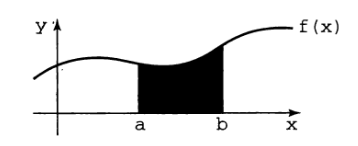
\includegraphics[scale=0.4]{img/integral.png}

Ci sono due modi fondamentali per approssimare il valore di un integrale. Uno è quello di dividere l'intervallo da \textit{a} a \textit{b} in un numero fisso di sottointervalli e poi approssimare l'area di ogni sottointervallo usando qualcosa come la regola trapezoidale o la regola di Simpson.

Il secondo modo per approssimare un integrale è quello di utilizzare il paradigma \textit{divide et impera}e un numero variabile di sottointervalli. In particolare, prima si calcola il punto medio \textit{m} tra \textit{a} e \textit{b}. Poi approssimare l'area di tre regioni sotto la curva definita dalla funzione \textit{f()}: quella da \textit{a} a \textit{m}, quella da \textit{m} a \textit{b} e quella da \textit{a} a \textit{b}. Se la somma delle due aree più piccole è entro una certa  tolleranza \textit{epsilon} accettabile dell'area più grande, allora l'approssimazione è considerata abbastanza buona. In caso contrario, il problema più grande - da \textit{a} a\textit{ b} - viene diviso in due sotto problemi - da \textit{a} a \textit{m} e da \textit{m} a \textit{b} - e il processo viene ripetuto. Questo approccio è chiamato quadratura adattiva perché l'algoritmo si adatta alla forma della curva: più la curva è morbida, meno sono gli intervalli e quindi le ricorsioni.

Sostanzialmente è possibile applicare la programmazione concorrente quando sono usate tecniche del tipo divide-et-impera, con procedure che lavorano su sottoinsiemi diversi di dati, in quanto molto probabilmente esse sono indipendenti e quindi possono essere eseguite parallelamente.

Applicazioni reali: no, difficile da gestire, applicazioni dinamiche in quanto non so a priori quanti processi si creano, quante ricorsioni servono, quindi non posso ottimizzare in anticipo.
Fondamentalmente è difficile equilibrare il lavoro: le prestazioni buone le ottengo facendo \textit{load balancing} ovvero dividendo equamente il carico. Nei programmi ricorsivi ciò è difficile per la variabilità dei dati nelle suddivisioni che si ottengono (nei grafi).

\subsection{Producers and Consumers: Unix Pipes}
Un processo produttore calcola e produce un flusso di risultati. Un processo consumatore consuma un flusso di valori. Molti programmi sono sia produttori che consumatori. Essi funzionano bene quando inseriti in una \textit{pipeline} in cui il primo processo produce qualcosa che passa al successivo, il quale a sua volta lo elabora(consuma) e passa il risultato al successivo e così via.


\subsection{Client and Server}
\`{E} il pattern più diffuso. Un processo \textit{client} richiede un servizio, poi aspetta che la richiesta venga gestita. Un processo \textit{server} aspetta ripetutamente una richiesta, la gestisce e poi invia una risposta. C'è un flusso bidirezionale di informazioni: dal client al server e poi indietro.

La relazione tra un client e un server è l'analogo della programmazione concorrente della relazione tra il chiamante di una subroutine e la subroutine stessa. Inoltre, come una subroutine che può essere chiamata da più posti, un server tipicamente ha molti clienti.

Questo paradigma può essere implementato su un sistema shared-memory, in cui un file server sarebbe tipicamente implementato da un insieme di subroutine (per leggere, scrivere, ecc.) e strutture di dati che rappresentano i file (ad esempio, * descrittori di file). Così, l'interazione tra un processo client e un file sarebbe tipicamente implementata da chiamate di subroutine. Tuttavia, se un file è condiviso, è probabilmente importante che sia scritto al massimo da un processo client alla volta. D'altra parte, un file condiviso può tranquillamente essere letto simultaneamente da più client.
Inoltre puà essere implementato in n sistema distribuito, in cui client e server risiedono su macchine diverse e collegati in rete.

-----puoi aggiungere come vengono programmati client e server in base a dove viene implementato il paradigma.

\subsection{Peers}
Si parla di peers quando ci sono programmi distribuiti con tanti processi che più o meno eseguono tutti lo stesso codice e si scambiano messaggi. Questo paradigma è spesso utilizzato per implementare programmi paralleli che utilizzano il parallelismo iterativo, nel senso che ogni peer lavora su un sottoinsieme di dati e si sincronizzano (e.g. moltiplicazione matrici).

esempio: moltiplicazione di matrici ma come viene distribuita la memoria tra i peers? cioè ogni peers ha l'intera matrice a e b in memoria? o no?




%programmazione a variabili condivise
%shared memory più correttamente
%///////////////////////////////////////////////////////////////
%   capitolo 2
%///////////////////////////////////////////////////////////////
\section{Shared-variable programming}
\subsection{Concetti fondamentali}
\begin{itemize}
\item stato del programma: snapshot, istantanea che vede il valore di variabili, registri, program counter in un dato momento.
\item azioni atomiche: istruzione che in maniera indivisibile esamina o modifica lo stato del programma, senza che nessun'altra istruzione possa essere eseguita nel frattempo.
\item history/trace: sequenza di azioni atomiche, composta da stato iniziale, transizioni e stato finale.
\item Proprietà: attributo che è vero per ogni possibile storia di quel programma e quindi di tutte le esecuzioni del programma.\\
 L'esecuzione parallela può essere modellata come una storia lineare, perché l'effetto dell'esecuzione di un insieme di azioni atomiche in parallelo è equivalente alla loro esecuzione in un certo ordine seriale.
Ogni esecuzione di un CP produce un storia diversa, cioè si hanno diverse combinazioni di azioni atomiche. Questo perché non si conosce la velocità dei processi, stato di attività del processore, o perché i processori girano a velocità diverse. Evidente conseguenza è che non è detto che ogni storia sia corretta, ovvero che produce risultati giusti. Qui entra in gioco la sincronizzazione.
\end{itemize}

Il ruolo della sincronizzazione è quello di vincolare le storie che si possono verificare in maniera da ottenere solo storie desiderabili ai fini dei risultati e verificare le proprietà viste in seguito.
Forme di sincronizzazione sono: \textbf{mutua esclusione}, cioè rendere (far apparire) una sequenza di azioni atomica, indivisibile, e \textbf{sincronizzazione su condizione}, cioè ritardare l'esecuzione di un'azione finché non è vera una condizione.

\subsubsection{Proprietà}
\label{sec:prop-prog}
La proprietà fondamentale di un programma è che esso termini e faccia quello che deve fare correttamente.

Ci sono due tipi di proprietà: \textbf{safety e liveness}. Una proprietà di \textbf{safety} è quella in cui il programma non entra mai in un cattivo stato, cioè uno stato in cui alcune variabili hanno valori indesiderati.
Una proprietà di \textbf{liveness} è quella in cui il programma alla fine (sicuramente prima o poi succede: eventually) entra in uno stato buono, cioè uno stato in cui le variabili hanno valori desiderabili.

La \textbf{correttezza parziale} è un esempio di proprietà di sicurezza. Un programma è parzialmente corretto se lo stato finale è corretto, assumendo che il programma termini.
La \textbf{terminazione} è un esempio di proprietà di liveness. Un programma termina se ogni ciclo e chiamata di procedura termina - quindi, se la lunghezza di ogni storia è finita. La \textbf{correttezza totale} è una proprietà che combina la correttezza parziale e la terminazione: Un programma è totalmente corretto se termina sempre con una risposta corretta.
La mutua esclusione è un esempio di proprietà di safety in un programma concorrente. Il cattivo stato in questo caso sarebbe quello in cui due processi stanno eseguendo azioni in diverse sezioni critiche allo stesso tempo. L'eventuale ingresso in una sezione critica è un esempio di una proprietà di liveness in un programma concorrente.

\textit{Come si dimostra che un programma soddisfi certe proprietà?}
\begin{itemize}
\item operare a botte di testing/debugging, ma ciò non rappresenta una soluzione valida in quanto non si può analizzare ogni caso possibile (dati input molteplici e diversi). Il difetto del testing è che ogni test considera solo una storia di esecuzione, e un numero limitato di test è improbabile che dimostri l'assenza di cattive storie.
\item operational reasoning: tentare di fare un'analisi di tutti i possibili casi che si possono verificare. Ciò non è possibile poiché il numero di storie in un programma concorrente generalmente è enorme.
\item assertional reasoning: (analisi astratta), ragionare per asserzioni, forme logiche dei predicati usate per caratterizzare un insieme di stati del programma e.g. x > 0.
\end{itemize}

\subsection{Parallelizzazione}
Il requisito fondamentale per poter parallelizzare qualsiasi programma è che esso contenga parti indipendenti. Due parti sono dipendenti l'una dall'altra se una produce risultati di cui l'altra ha bisogno; questo può accadere solo se leggono e scrivono variabili condivise.
Quindi, due parti di un programma sono indipendenti se non leggono e scrivono le stesse variabili.
Più \textbf{precisamente}: due operazioni sono indipendenti se il \textit{write set} di ciascuna parte è disgiunta da entrambi i \textit{write set} e \textit{read set} dell'altra parte.

esempio slide, comando grep, libro pag 44/45

problema del comando grep
grep pattern filename

\begin{verbatim}
string line;
read a line of input from stdin into line;
while (!EOF) { # EOF is end of file
	look for pattern in line;
	if (pattern is in line)
		write line;
	read next line of input;
}
\end{verbatim}

Come parallelizzarlo?
Si può leggere la prossima linea di input mentre cerchiamo il pattern nella linea precedente:

\begin{verbatim}
string line;
read a line of input from stdin into line;
while (!EOF) {
co look for pattern in line;
if (pattern is in line)
write line;
// read next line of input into line;
oc;
}
\end{verbatim}

I due processi (nello statement co) sono indipendenti? La risposta è no, perché il primo processo legge e il secondo processo vi scrive. Quindi, se il secondo processo gira più velocemente del primo, sovrascriverà la linea prima che venga esaminata dal primo processo.

Supponiamo che il secondo processo legga in una variabile diversa da quella che viene esaminata dal primo processo:
\begin{verbatim}
string linel1, line2;
read a line of input from stdin into linel;
while (!EOF) {
co look for pattern in linel;
if (pattern is in linel)
write linel;
/ / read next line of input into line2;
oc;
}
\end{verbatim}

Ora, i due processi stanno lavorando su linee diverse, che sono memorizzate in variabili line1 e line2. Quindi, i processi possono essere eseguiti simultaneamente. Ma è il programma di cui sopra è corretto? Ovviamente no, perché il primo processo guarda continuamente line1, mentre il secondo processo legge continuamente line2, che non viene mai esaminata.
La soluzione è relativamente semplice: scambiare i ruoli delle linee alla fine di ogni iterazione del ciclo, in modo che il primo processo esamini sempre l'ultima linea letta e il secondo processo legga sempre in una variabile diversa da quella esaminata. Il seguente programma realizza questo:

\begin{verbatim}
string line1, line2;
read a line of input from stdin into linel;
while (! EOF) {
co look for pattern in linel;
if (pattern is in linel)
write linel;
/ / read next line of input into line2;
oc;
linel = line2;
}
\end{verbatim}


Il programma concorrente di cui sopra è corretto, ma è piuttosto inefficiente perché: aggiunge l'operazione di copia, che generalmente lavora su tanti caratteri, il che produce overhead; ad ogni iterazione del while  due processi vengono creati, eseguiti e distrutti.
La soluzione è fare una copia più efficiente, ovvero leggere le linee, memorizzarle in un array e accedendovi cambiando l'indice; e invece di avere un co nel while usare un while nel co, così da creare i processi una sola volta evitando overhead.

\begin{verbatim}
string buffer; # contains one line of input
bool done = false; # used to signal termination
co # process 1: find patterns
string linel;
while (true) {
wait for buffer to be full or done to be true;
if (done) break;
linel = buffer;
signal that buffer is empty;
loot for pattern in linel;
if (pattern is in linel)
write linel;
}
// # process 2: read new lines
string line2;
while (true) {
read next line of input into 1 ine2;
if (EOF) {done = true; break; }
wait for buffer to be empty;
buffer = line2;
signal that buffer is full;
}
oc;
\end{verbatim}


Esso funziona come il modello produttore/consumatore e i due processi comunicano tramite un buffer il quale indica il tipo di sincronizzazione richiesta.

\subsection{Sincronizzazione: valore massimo in un array}
Programma sequenziale per il calcolo del massimo:
\begin{verbatim}
int m=0;
for [i=0 to n -1] {
 if (a[i]>m)
 m=a[i];
} 
\end{verbatim}

Per parallelizzarlo si può mettere l'operatore \textit{co} al loop, ma in questo modo il programma sarà scorretto, in quanto i processi non sono indipendenti: ognuno legge e scrive la variabile \textit{m}.

Nel passo successivo vengono usate, linguaggio mpd del libro, le parentesi angolari che definiscono che il codice al loro interno viene eseguito atomicamente.
\begin{verbatim}
int m = 0;
co [i = 0 to n-1]
<if (a[i] > m)
m = a[i];>
\end{verbatim} 
Così il programma è corretto, tuttavia esso sarà comunque sequenziale perché le if sono eseguite atomicamente con la differenza che gli elementi dell'array sono esaminati in ordine arbitrario(senza norma).

La chiave della questione è assicurare che gli aggiornamenti di \textit{m} siano atomici:
\begin{verbatim}
int m = 0;
co [i = 0 to n-1]
if (a[i] > m)
<m = a[i];>
\end{verbatim} 
Neanche questa versione è corretta perché questo programma è in realtà lo stesso del primo programma concorrente: ogni processo potrebbe confrontare il suo valore di a con m e poi aggiornare il valore di m.

Il miglior modo per risolvere il problema è combinare i due programmi precedenti:
\begin{verbatim}
int m = 0;
co [i = 0 to n-1]
if (a[i] > m) # check the value of m
<if (a[i] > m) # recheck the value of m
m = a[i];>
\end{verbatim}

il primo check fa una scrematura dei valori di a[i] che sono eleggibili a diventare massimi e scarta i valori bassi, e prima di memorizzare \textit{m} si rifà il check sul valore di m in maniera atomica. Il check viene rifatto poiché i processi che lavorano su m sono molteplici.

\subsection{Atomic Actions}
possiamo vedere l'esecuzione di un programma concorrente come un interleaving delle azioni atomiche eseguite dai singoli processi. Quando i processi interagiscono, non tutti gli intrecci sono accettabili. Il ruolo della sincronizzazione è quello di prevenire interleaving indesiderati: 
\begin{itemize}
\item mutua esclusione: combinando azioni atomiche a grana fine in azioni a grana grossa (composte).
\item sinc su condizione: ritardando l'esecuzione di un processo finché non è verificata la condizione.
\end{itemize}

Ricordiamo che un'azione atomica fa una trasformazione di stato indivisibile. Questo
significa che qualsiasi stato intermedio che potrebbe esistere nell'implementazione dell'azione
non deve essere visibile ad altri processi. Un'azione atomica a grana fine è una
che è implementata direttamente dall'hardware su cui un programma concorrente
esegue.

L'istruzione di assegnazione sembra essere atomica nei programmi sequenziali, generalmente non è così nei programmi concorrenti perché può essere implementato da una sequenza di istruzioni in linguaggio macchina.

int y = 0, z = 0;
co x = y+z; // y = 1; z = 2; oc;

x potrà valere: 0, 1, 3 dipende da quando il secondo processo (assegnazione y,z) verrà eseguito. Può accadere che x sarà 2. Come? anomalia, prendo i valori di y e z in \textbf{due istanti diversi}, (cit. un valore di 30 anni prima e uno attuale), il che rende le operazioni \textbf{non atomiche}

\subsubsection{Hardware model usato dal libro}
Il modello hardware cui fa riferimento il libro dice che:
\begin{itemize}
\item i tipi di base(int) vengono conservati in memoria e lette e scritte come azioni atomiche.
\item i valori su cui si opera vengono caricati nei registri, elaborati nei registri, e i risultati rimemorizzati in memoria.
\item il processore del modello del libro utilizza un set di registri proprietari per ogni processo, cioè ad ogni cambio di contesto c'è il salvataggio dei registri che poi verranno recuperati alla successiva esecuzione del processo.
\item tutti i risultati intermedi vengono salvati in registri o in stack.
\end{itemize}

\subsubsection{Disjointness Requirement}
Qual è il requisito per cui un'espressione può essere vista come atomica?
Con questo modello di macchina, se un'espressione \textit{e} in un processo non fa riferimento a una
variabile alterata da un altro processo, la valutazione dell'espressione \textbf{sembrerà essere
atomica}, anche se richiede l'esecuzione di diverse azioni atomiche a grana fine. 

la valutazione dell'espressione \textbf{apparirà come atomica} se valgono queste due proprietà: \textbf{(1)} nessuno dei valori da cui \textit{e} dipende potrebbe cambiare mentre
\textit{e} viene valutato, e \textbf{(2)} nessun altro processo può vedere qualsiasi valore temporaneo che
potrebbero essere creati mentre l'espressione viene valutata. 
Quindi un'espressione viene valutata come se fosse atomica se non utilizza variabili che vengono scritte e modificate da un altro processo.

Allo stesso modo, se un assegnazione \textit{x = e} in un processo non fa riferimento a nessuna variabile alterata da un altro processo - per esempio, fa riferimento solo a variabili locali - allora l'esecuzione dell'assegnazione sembrerà essere atomica.

Il problema nasce quando il secondo processo modifica due variabili condivise, quindi il primo può ricevere  un valore vecchio e uno nuovo (dato il timing dei processi, scheduling), ed è questa la situazione da evitare, che non accadrebbe se l'operazione fosse atomica.

Sfortunatamente, la maggior parte delle istruzioni in programmi concorrenti che fanno riferimento a
variabili condivise non soddisfano il \textbf{requisito di disgiunzione} spiegato sopra. 
Tuttavia, un requisito più debole è spesso soddisfatto.

\subsubsection{Proprietà at-most-once}
\`{E} un requisito più debole del precedente che comunque garantisce che la valutazione dell'espressione e l'eventuale assegnazione possano essere considerate atomiche.
Riferimento critico in un'espressione è un riferimento ad una variabile che viene modificata da un altro processo.

Un'espressione soddisfa la proprietà at-most-once se:\\
- contiene al massimo un riferimento ad una variabile semplice modificata da un altro processo (riferimento critico) AND\\
- si riferisce a quella variabile al massimo una volta\\

L'istruzione di assegnazione \textit{x=e} soddisfa la proprietà at-most-once se:\\
- \textit{e} contiene al massimo un riferimento critico ad una variabile semplice AND\\
\textit{x} non viene letto (referenziato) da un altro processo\\
OR\\
- \textit{e} non contiene alcun riferimento critico, quindi \\
\textit{x} può essere letto da altri processi\\

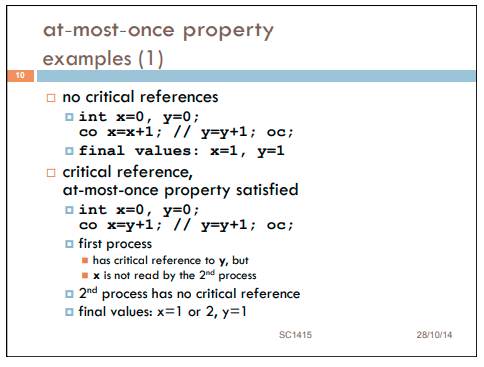
\includegraphics[scale=0.65]{img/mostonce.png} \\
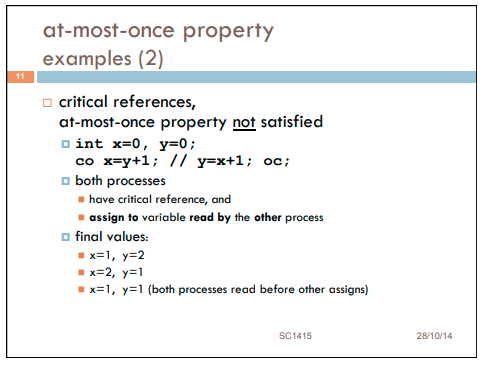
\includegraphics[scale=0.65]{img/mostonce2.png} 
qui, ultima slide, non vale la proprietà at most once quindi le operazioni non sono eseguite come se fossero atomiche e possono verificarsi situazioni anomale (lettura di valori vecchi e nuovi)

se l'espressione o la dichiarazione di assegnazione non soddisfa
la proprietà at-most-once, potremmo ancora volere l'esecuzione atomica. Per far ciò bisogna creare un'azione atomica \textbf{coarse-grained}, di grana grossa, composta da più istruzioni, ed eseguirle come se fossero atomiche, utilizzando le parentesi angolari o primitive di sincronizzazione.


\subsection{Sincronizzazione}
La sincronizzazione viene utilizzate per prevenire interleaving indesiderati. Ciò lo si ottiene con: 
\begin{itemize}
\item mutua esclusione, che combina azioni atomiche a grana fine in azioni atomiche di grana grossa, insomma fa apparire roba non atomica come se fosse atomica. (e.g. bonifico bancario: mentre trasferisco i soldi non si deve vedere lo stato in cui i soldi non sono né su uno né sull'altro conto; puntatori, insert e remove).
\item sinc su condizione, ritarda esecuzione di un processo finché non è vera la condizione.
\end{itemize}

\subsection{AWAIT}
Notazione linguaggio mpd: \begin{verbatim} parentesi angolari < >\end{verbatim}
await statement: \begin{verbatim} <await (B) S; >\end{verbatim}
Con questo statement viene garantita la mutua esclusione, ma viene introdotta anche la sincronizzazione su condizione: S è una sequenza di statement mentre B è la condizione di ritardo.
Lo stato interno di S non è visibile agli altri processi, ma sarà visibile solo lo stato finale, e nessun altro processo può modificare le variabili referenziate in B o S mentre lo statement è in esecuzione.

\textbf{esempio} con variabile semaforica: \begin{verbatim} <await (s > 0) s = s – 1;> \end{verbatim} 
 - actually P operation on semaphore s \\

 $ in questo corso si usa la notazione p e v per i semafori $

\paragraph{mutual exclusion} \begin{verbatim}<S;>\end{verbatim}
\begin{verbatim}<x=x+1;y=y+1;>\end{verbatim}
outside world cannot see state when x is incremented, but y not yet \\

se S è un'istruzione atomica o è un'assegnazione che soddisfa la proprietà at-most-once(appare come atomica), \begin{verbatim}<S;> è equivalente a S\end{verbatim} 

\paragraph{condition sync}
\begin{verbatim} <await (B) ; >\end{verbatim}
manca la lista di statement a destra, si ha semplicemente la sincronizzazione su condizione senza esecuzione di altre istruzioni, aspetta che un altro processo modifichi B per sbloccare il processo corrente e andare avanti.
 \begin{verbatim}e.g. <await (count > 0);>\end{verbatim}

Inoltre, se B soddisfa la proprietà at-most-once lo statement \begin{verbatim} <await (B) ; >\end{verbatim} può essere implementato con un \begin{verbatim} while (not B); # chiamato spin loop\end{verbatim}


\section{Semantica assiomatica: concetti chiave e terminologia}
Il concetto chiave da sapere di questa sezione è rappresentato dalle triplette.\\ \\
\textit{Reprise: Come si dimostra che un programma soddisfi certe proprietà?}
\begin{itemize}
\item operare a botte di testing/debugging, ma ciò non rappresenta una soluzione valida in quanto non si può analizzare ogni caso possibile (dati input molteplici e diversi). Il difetto del testing è che ogni test considera solo una storia di esecuzione, e un numero limitato di test è improbabile che dimostri l'assenza di cattive storie.
\item operational reasoning: tentare di fare un'analisi di tutti i possibili casi che si possono verificare. Ciò non è possibile poiché il numero di storie in un programma concorrente generalmente è enorme.
\item assertional reasoning: (analisi astratta), ragionare per asserzioni, forme logiche dei predicati usate per caratterizzare un insieme di stati del programma e.g. x > 0.
\end{itemize}

useremo il ragionamento assertivo frequentemente nel resto del testo.
La base per il ragionamento assertivo è quella che viene chiamata \textbf{logica di programmazione}:
un sistema logico formale che facilita la formulazione di affermazioni precise sull'esecuzione del programma.

\textbf{un sistema logico formale è} un'astrazione matematica, ossia un'insieme di simboli e relazioni fra essi, in particolare è costituito da:
\begin{itemize}
\item insieme di simboli
\item insieme di formule, costruite con i simboli
\item insieme di assiomi, formule vere a priori
\item insieme di regole di inferenza (deduzione), permettono a partire da certe ipotesi di estrarre/dedurre una conclusione
\end{itemize}
Se tutte le ipotesi sono vere, allora possiamo dedurre che la conclusione è anche vera.

\textbf{Teorema}: sequenza di linee.
\textbf{Proof (prova)}: sequenza di linee che sono assiomi o derivabile mediante regole di inferenza.

tali sistemi logici sono di particolare interesse dove formule rappresentano degli statement riguardanti un certo dominio, il che significa che le formule hanno una certa interpretazione e i teoremi sono statement veri.
L'interpretazione della logica permette di mappare ogni formula come vera o falsa.

\textbf{Sound logic}: logica solida nei riguardi di un'interpretazione, se tutti gli assiomi sono solidi/sound, ovvero mappati a true, e se tutte le regole di inferenza sono sound, ovvero se le conclusioni sono mappate a true assumendo che anche tutte le ipotesi sono mappate a true.
In pratica tutti i teoremi statement sono mappati a true nel dominio. Se così è, l'interpretazione è chiamata \textit{modello} per quella logica.

\textbf{Complete logic} nei riguardi di un'interpretazione, se ogni formula può essere dimostrabile nella logica.
\newpage
Considerazioni:\\
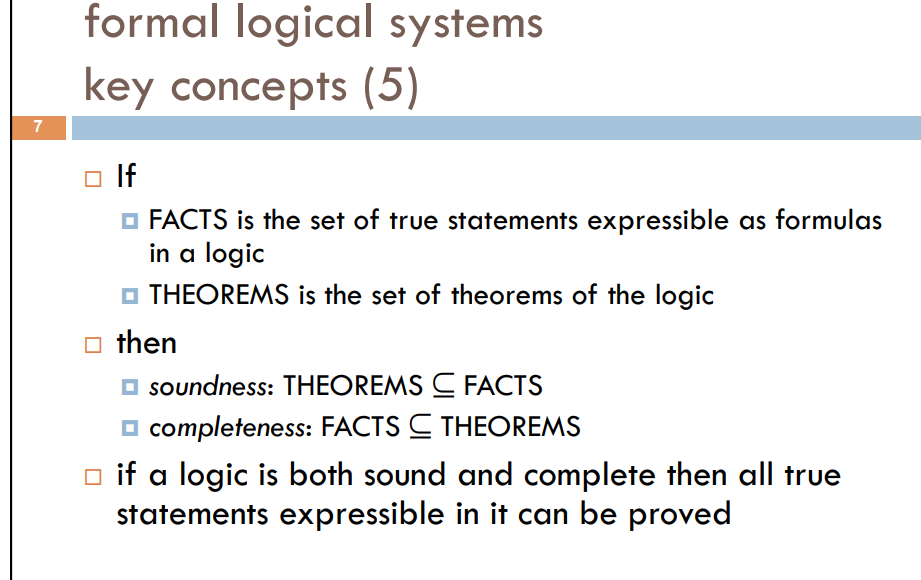
\includegraphics[scale=0.45]{img/considerazioni.png} \\
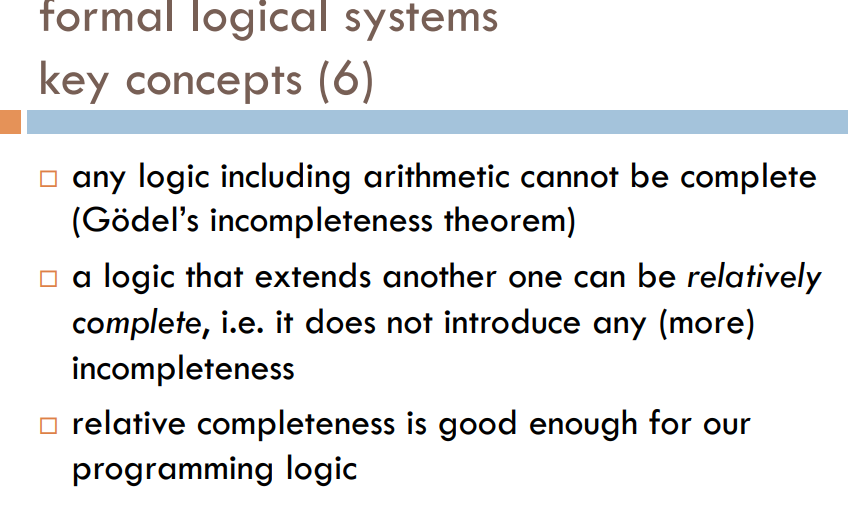
\includegraphics[scale=0.45]{img/considerazioni2.png} \\
\newpage
Una \textbf{programming logic} è un sistema logico formale che consente di affermare e dimostrare le proprietà del programma.
La logica di Andrews chiamata PL è composta da: simboli(predicati, parentesi, statement), formule(triple {P} S {Q}), assiomi e regole di inferenza.

\textit{interpretazione di una tripla}: la tripla {P} S {Q} è vera se, ogniqualvolta l'esecuzione di S è iniziata in uno stato che soddisfa P e l'esecuzione di S termina, lo stato risultante soddisfa Q.
\textit{vera P, dopo esecuzione di S, Q è vera.}

\paragraph{Proprietà}: attributi veri per qualsiasi storia, qualsiasi incastro degli eventi.
Si dividono in:
\begin{itemize}
\item proprietà di safety: garantiscono che un programma non si porti mai in un bad state; \textit{partial correctness} stato finale corretto se il programma termina.
\item proprietà di liveness: garantiscono che prima o poi un programma si porta in uno stato desiderato(good state); \textit{termination} ogni ciclo, procedura, storia ecc termina.
\item total correctness=partial correctness+termination; il programma termina sempre con risposta corretta, stato desiderato.
\end{itemize} 

In una tripla, i predicati P e Q sono spesso chiamati asserzioni, perché affermano che lo stato del programma deve soddisfare il predicato affinché l'interpretazione della tripla sia vera.
Le asserzioni sono stati accettabili del programma, P è precondizione, Q postcondizione.\\
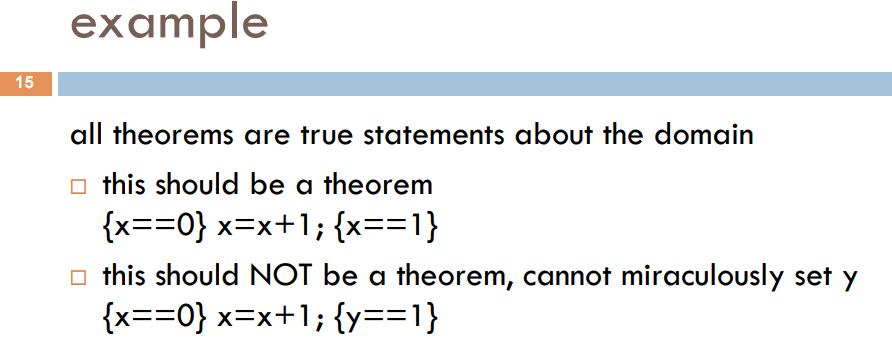
\includegraphics[scale=0.45]{img/theorem.png} \\

\paragraph{Skip axiom} {P} skip {P}.
skip non cambia nessuna variabile. Quindi, se un predicato è vero prima dell'esecuzione di skip, rimane
true quando skip termina.

\paragraph{Assegnazione assioma\\}
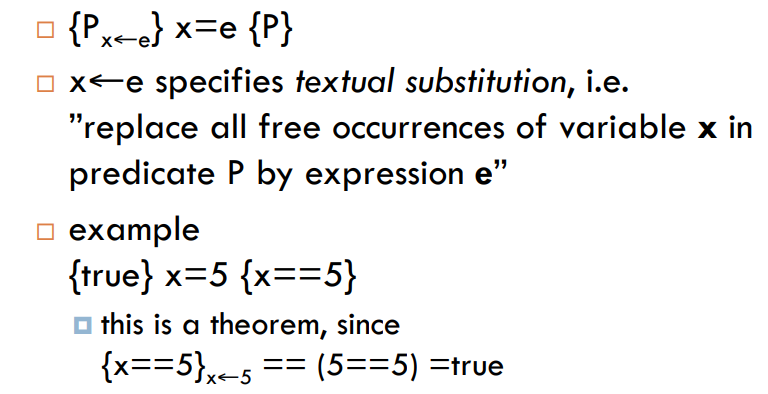
\includegraphics[scale=0.45]{img/ax.png} \\ \\ \\
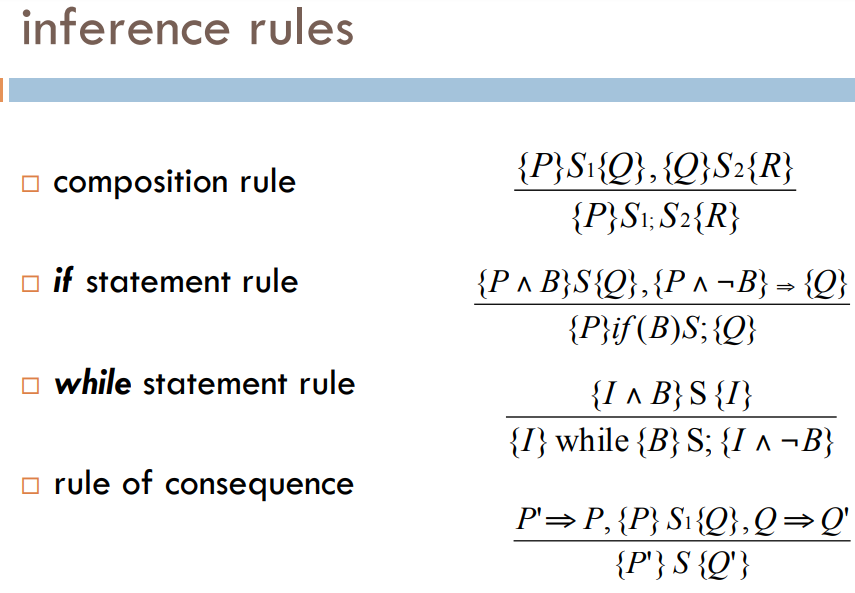
\includegraphics[scale=0.45]{img/inference.png} \\ \\ \\
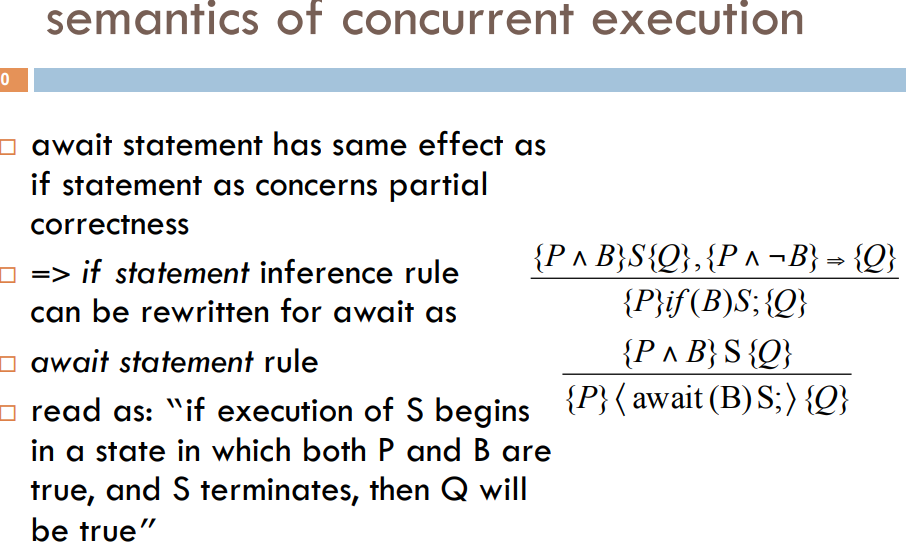
\includegraphics[scale=0.45]{img/inf2.png} \\ \\ \\

\paragraph{Interferenza} un processo attraverso un'assegnazione invalida un'asserzione nell'altro.
le asserzioni caratterizzano ciò che un processo assume essere vero prima e dopo ogni affermazione (pre e post condizione)\\
Esempio: un processo assegna a una variabile condivisa e quindi invalida il presupposto di un altro processo.
\begin{verbatim}
{x==0}
co <x=x+1;> // <x=x+2;> oc
{x==3}
\end{verbatim}

Con la proof outline si può dimostrare la correttezza del programma, cioè si parte dalle asserzioni e si deve dimostrare che tutte le triplette risultanti siano vere.
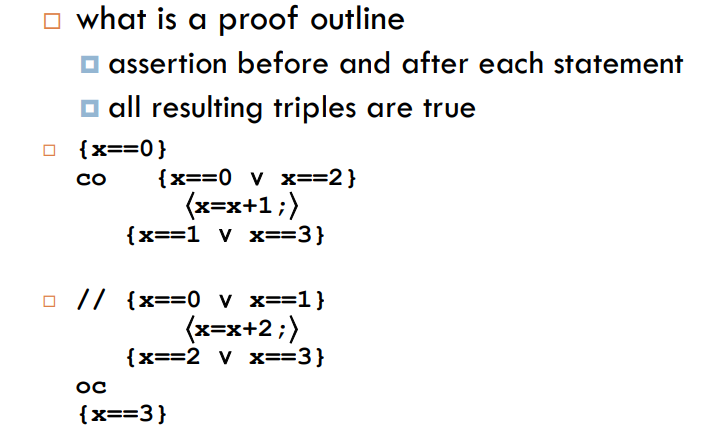
\includegraphics[scale=0.45]{img/proof.png} \\ \\ \\

\paragraph{noninterference}
le \textbf{azioni di assegnazione} possono stare da sole nello statement oppure stare all'interno di uno statement \textit{await}.
una \textit{asserzione critica} è una pre o post condizione che non si trova in uno statement \textit{await} cosicché potrebbe essere cambiata da altro processo.

\paragraph{avoiding interference}
Un insieme di processi è esente da interferenze se no l'azione di assegnazione in un processo interferisce con qualsiasi affermazione critica in un altro.

Tecniche per evitare interferenza:
\begin{itemize}
\item variabili disgiunte, già visto abbondantemente. Capita di rado.
\item asserzioni indebolite: 
\item invarianti globali
\item sincronizzazione
\end{itemize}

\subsection{Proprietà}
Si riprendano i concetti di proprietà~\vref{sec:prop-prog}.

In un programma concorrente valgono le stesse proprietà che valgono nei programmi sequenziali, ma se ne applicano anche altre. In particolare per un CP due importanti proprietà di \textit{safety} sono la mutua 
esclusione e l'assenza di deadlock. Per la mutua esclusione, il bad state è avere più di un processo che esegue sezioni critiche allo stesso tempo.
Per il deadlock, il bad state è avere tutti i processi in attesa di condizioni che non si verificheranno mai.
Le proprietà di \textit{liveness} sono influenzate dalle politiche di \textit{scheduling}, che determinano quali azioni atomiche ammissibili sono le prossime ad essere eseguite.
Esempi di proprietà di liveness dei programmi concorrenti sono che un processo alla fine riuscirà ad entrare in una sezione critica, che una richiesta di servizio alla fine sarà onorata, o che un messaggio alla fine raggiungerà la sua destinazione.

\subsubsection{Dimostrare le proprietà di safety}
Ogni azione che un programma compie è basata sul suo stato(registri, variabili, ecc). 
\paragraph{safety}Se un programma non riesce a soddisfare una proprietà di safety, ci deve essere qualche stato "cattivo/bad" che non riesce a soddisfare la proprietà.
Per esempio, se la proprietà di mutua esclusione non tiene, ci deve essere qualche stato in cui due (o più) processi sono contemporaneamente nelle loro sezioni critiche.
O se i processi si bloccano, ci deve essere qualche stato in cui il deadlock si verifica.

i metodi per provare le prop di safety sono due:
\subparagraph{1} Sia BAD un predicato che caratterizza un cattivo stato. Allora un programma soddisfa la proprietà di safety associata se BAD è falso in ogni stato in ogni possibile storia del programma. Dato il programma S, mostrare che BAD non è vero in ogni stato richiede di dimostrare che non è vero nello
stato iniziale, nel secondo stato, e così via, dove lo stato viene cambiato come risultato dell'esecuzione di azioni atomiche.
\subparagraph{2} In alternativa, e in modo più potente, se un programma non deve mai essere in uno stato BAD allora deve essere sempre in uno stato GOOD, dove GOOD è equivalente a BAD. Quindi, un modo efficace per garantire una proprietà di sicurezza è specificare BAD, poi negare BAD per ottenere GOOD, poi assicurarsi che GOOD sia un invariante globale predicato che è vero in ogni stato del programma. La sincronizzazione può essere usata - come abbiamo visto e vedremo molte altre volte nei capitoli successivi - per assicurare che un predicato sia un invariante globale.

\paragraph{liveness}
La maggior parte delle proprietà di liveness dipende dalla \textit{fairness}, che si occupa di garantire che i processi abbiano la possibilità di procedere, indipendentemente da ciò che fanno gli altri. Ogni processo esegue una sequenza di azioni atomiche. Un'azione atomica in un processo è \textbf{eleggibile} se è la prossima azione atomica nel processo che potrebbe essere eseguita.
Quando ci sono diversi processi, ci sono diverse azioni atomiche eleggibili. Una politica di scheduling determina quale sarà eseguita per prima. Questa sezione definisce tre gradi di fairness che una politica di scheduling potrebbe fornire.
Ricordiamo che un'azione atomica incondizionata è quella che non ha una condizione di ritardo.

\subparagraph{Unconditional Fairness} Una politica di scheduling è incondizionatamente equa se
ogni azione atomica incondizionata che è ammissibile viene eseguita prima o poi.\\
on a single processor -> round-robin\\
on multiprocessor -> parallel execution

\paragraph{Weak Fairness} Una politica di programmazione è debolmente equa se (1) è incondizionatamente equa, e (2) ogni azione atomica condizionata che è eleggibile viene eseguita alla fine, assumendo che la sua condizione \textbf{diventi vera e poi rimane vera} finché non viene vista dal processo che esegue l'azione atomica condizionata.

\paragraph{Strong Fairness} Una politica di scheduling è fortemente equa se (1) è incondizionatamente equa, e (2) ogni azione atomica condizionata che è eleggibile è eseguita prima o poi, assumendo che la sua condizione sia infinitamente spesso vera.

le politiche pratiche di programmazione non sono Strongly Fair !!!

\section{Lock and Barriers}


\subsection{Problema della sezione critica}
Il problema della sezione critica è uno dei classici problemi di programmazione concorrente. È stato il primo problema ad essere studiato estensivamente e rimane di interesse dato che la maggior parte dei programmi concorrenti hanno sezioni critiche di codice. Inoltre, la soluzione del problema può essere usata per implementare \textit{statement await} arbitrari.
Questa sezione definisce il problema e sviluppa una soluzione a grana grossa.
Nel problema della sezione critica, \textit{n} processi eseguono ripetutamente una sezione critica e poi
una sezione non critica di codice. La sezione critica è preceduta da un protocollo di entrata e seguita da un protocollo di uscita. Quindi, assumiamo qui che i processi abbiano la seguente forma:
process CS[i = 1 to n] {
while (true) {
entry protocol;
critical section;
exit protocol;
noncritical section;
}
}

Ogni sezione critica è una sequenza di istruzioni che accedono a qualche oggetto condiviso.
Ogni sezione non critica è un'altra sequenza di istruzioni.
Si assume come ipotesi fondamentale che un processo che vuole entrare in sezione critica prima o poi ne uscirà.
L'obiettivo è progettare un protocollo di ingresso e uscita dalla sezione critica che soddisfi le seguenti proprietà:
\begin{itemize}
\item Mutua Esclusione. Al più un processo alla volta esegue la sua sezione critica.
\item Assenza di Deadlock. Se ci sono due o più programmi che vogliono entrare in SC, almeno uno vi entrerà
\item Assenza di ritardo non necessario. Se un processo sta cercando di entrare nella sua sezione critica
e gli altri processi stanno eseguendo le loro sezioni non critiche o sono terminati, al primo processo non viene impedito di entrare nella sua sezione critica.
\item Eventual Entry(prima o poi ingresso in SC). Un processo che sta tentando di entrare nella sua sezione critica alla fine ci riuscirà.
\end{itemize}

\subsubsection{Soluzione}
In linguaggio mpd basta usare le parentesi angolari, usando l'await statement. Ma come sono implementate davvero?

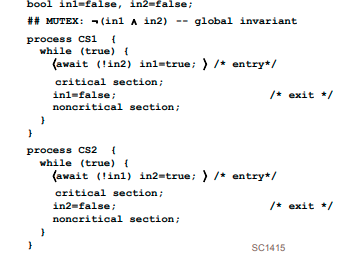
\includegraphics[scale=1]{img/cs.png} \\
Questo vale per due processi che vogliono entrare in sezione critica; per \textit{n} processi che vogliono entrarvi, basta sapere se la sez cr è libera o occupata usando la variabile \textit{lock == in1 or in2}.\\

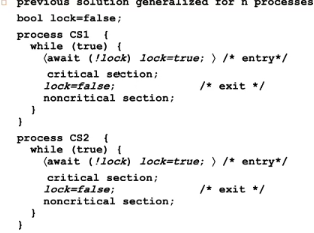
\includegraphics[scale=1]{img/cs2.png} \\

\subsubsection{Test and Set TS}
Resta da implementare l'await: \begin{verbatim} <await (!lock) lock=true; >\end{verbatim}

quasi tutte le macchine hanno qualche istruzione speciale per implementare le azioni di sopra, azione che sono garantite essere atomiche anche in ambienti multiprocessore.
\begin{verbatim}
Test-and-Set (TS)
bool TS (bool lock) {
 <bool initial=lock /* save initial value */
 lock=true; /* set lock */
 return initial; > /* return initial value */
}
\end{verbatim}
TS accetta una variabile \textit{lock} condivisa come argomento e restituisce un risultato booleano. Come azione atomica, TS legge e salva il valore di lock, imposta lock su true, quindi restituisce il valore iniziale salvato di lock. 

Poiché tutti i processi eseguono gli stessi protocolli, la soluzione come mostrato funziona per qualsiasi numero di processi. Quando una variabile di lock viene utilizzata come nel codice seguente è tipicamente chiamata \textbf{spin lock}. Questo perché i processi sono in loop (spinning, rotazione) in attesa che il lock venga cancellato. 

\begin{verbatim}
Soluzione alla sezione critica con spin lock e TS
bool lock=false; /* shared lock */
process CS [i=1 to n] {
 while (true) {
 while (TS(lock)) skip; /* entry protocol */
 critical section;
 lock=false; /* exit protocol */
 noncritical section;
 }
} 
\end{verbatim}

Non sono garantite tutte le proprietà, ma sicuramente entra in SC un processo per volta.
in una soluzione spin-lock del problema della sezione critica, il protocollo di uscita dovrebbe semplicemente resettare le variabili condivise ai loro valori iniziali

Questa soluzione funziona, ma male:

\paragraph{Problema del hotspot}
Perché \textit{lock} è una variabile condivisa e ogni processo ritardato continua a fargli riferimento. Ciò è detto \textit{hot spot} e causa contesa di memoria che abbassa notevolmente le performance.
Inoltre, l'istruzione ts scrive in lock ogni volta che viene eseguita, anche quando il valore di lock non cambia. Dal momento che multiprocessori a memoria condivisa utilizzano le cache per ridurre il traffico verso la memoria primaria, questo rende ts significativamente più costosa di un'istruzione che legge semplicemente una variabile condivisa. Perché quando una variabile è scritta da un processore, le cache degli altri devono essere invalidate se contengono una copia della variabile condivisa.

\paragraph{Test-and-Test-andSet protocol}
La contesa della memoria e l'overhead di invalidamento della cache possono essere entrambi ridotti con la modifica del protocollo di ingresso.
\begin{verbatim}
bool lock = false;
process CS[i = 1 to n] {
while (true) {
while (lock) skip;
while (TS(lock)) {
while (lock) skip;
}
critical section;
lock = false;
noncritical section;
}
}
\end{verbatim}

Questo è chiamato protocollo Test-and-Test-and-Set perché un processo si limita a testare lock finché non c'è la possibilità che ts possa avere successo. Nei due aggiuntivi loop, lock viene solo esaminato, quindi il suo valore può essere letto(e non scritto!) da una cache locale senza interessare altri processori. La contesa della memoria è così ridotta, ma non la fa scomparire. In particolare, quando il lock è azzerato almeno uno ed eventualmente tutti i processi ritardati eseguiranno ts, anche se solo uno può procedere.

\subsubsection{Implementa Await Statement}
Sostituisco le parentesi angolari con i protocolli CSenter e CSexit.
Ora rimane da implementare la condizione: 
\begin{verbatim}
CSenter;
while (!B) { CSexit; Delay; CSenter; }
S;
CSexit;
\end{verbatim}
la condizione è rappresentata dal while, ma, trovandosi il processo in sezione critica, essa non può essere modificata da altri processi poiché non possono entrare anch'essi in SC. Così, se la condizione non è verificata, si fa uscire il processo dalla sezione critica dando un intervallo di tempo ad altri processi per modificare B, e poi rientra in SC.

Tutte le soluzione precedenti sono basate sullo spin lock; questo metodo assicura la mutua esclusione, l'assenza di deadlock, evita ritardi non necessari. Tuttavia richiede uno scheduler strongly fair per assicurare l'entrata in SC, ma tale scheduler non esiste. Esiste il weakly fair.

Soluzioni con weakly fair per quest'ulteriore problema sono rappresentate da:
\begin{itemize}
\item tie-breaker algo
\item ticket algo
\item bakery algo
\end{itemize}

\subsubsection{Tie-Breaker Algorithm}
I problema: bisogna assicurarsi che non ci sia un processo che monopolizza la SC, altrimenti non è garantita l'eventual entry. Per ottenere una soluzione \textit{fair} i processi dovrebbero fare a turno per entrare in SC.

L'algoritmo del Tie-breaker aggiunge una variabile \textit{last} che indica chi è stato l'ultimo processo ad entrare in SC. Quindi quando si trovano due processi con \textit{in=true}, cioè pronti ad entrare in SC, in base a \textit{last} si decide chi vi entrerà.

\textit{il libro fa tutto l'escursus di come arriva alla soluzione corretta tramite codici parzialmente corretti.}

Funziona solo su due processi.\\
Su n processi è complicata.


\textbf{\textit{lo statement await è implementabile con lo spin loop solo se la condizione soddisfa la proprietà at most once}}\\

%///////////
%  The Art of Computer Programming Libro di Donald Knuth (Bibbia) 
%///////////

\subsubsection{Ticket Algorithm: ding dong. serviamo il numero x}
\marginpar{videolezione 2021-10-06}
Processi, come i clienti della salumeria, vengono serviti/entrano in SC in ordine di arrivo, con l'ordine definito dal biglietto/ticket ottenuto.
\begin{verbatim}
int number = 1, next = 1, turn[l:n] = ([n] 0);
## predicate TICKET is a global invariant (see text)
process CS[i = 1 to n] {
while (true) {
<turn[i] = number; number = number + 1;>
<await (turn[i] == next);>
critical section;
<next = next + 1;>
noncritical section;
}
}
\end{verbatim}

Per entrare nella sua sezione critica, il processo CS[i] prima imposta turn[i] al valore corrente di \textit{number} e poi lo incrementa. Si tratta di una singola azione atomica(parentesi angolari) per assicurare che i clienti estraggano numeri unici. Al completamento della sua sezione critica, CS[i] incrementa \textit{next}, di nuovo come un'azione atomica.\\
global invariant che formalizza la situazione:\\
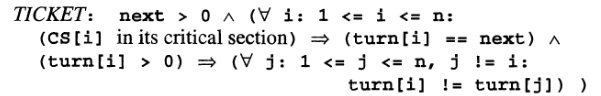
\includegraphics[scale=0.4]{img/ticket.png} \\

Visto che i valori di \textit{turn} sono unici c'è assenza di deadlock e assenza di ritardo non necessario perché un processo che non vuole entrare in SC avrà \textit{turn=0} quindi non viene preso in considerazione.
Infine, se lo scheduling è weakly fair, l'algoritmo assicura l'ingresso, perché una volta che una condizione di ritardo diventa vera, rimane vera.
Problema se l'algoritmo gira per molto tempo le variabili \textit{number e next} crescono e potrebbero causare overflow.

Problema: la prima azione atomica dell'algoritmo che legge e incrementa(FA Fetch-and-Add) \textit{number} è difficile da implementare se non si ha un processore che lo fa atomicamente. In sostanza sui processori che non dispongono di tale capacità (nostri), l'istruzione deve essere implementata seguendo un altro approccio: \begin{verbatim}
turn[i] = number; <number = number +1 >
\end{verbatim} 
Questo assicura che \textit{number} venga incrementato correttamente ma non che ci siano valori unici di number.
Le altre azioni atomiche si implementano facilmente(await con busy-waiting loop perché solo next è condivisa//next++ con load and store perché soloun processo alla volta farà l'exit protocol).

Senza FA, si utilizza la sezione critica con: \begin{verbatim}CSenter e CSexit: CSenter; turn[i] = number; number = number+1; CSexit;\end{verbatim}

\subsubsection{Bakery Algorithm}
Algoritmo \textit{fair} che non occorre di istruzioni speciali come FA.
Concetto chiave: il cliente col numero più basso viene servito prima, gli altri si confrontano tra di loro(scusate chi è l'ultimo?). Senza variabile globale \textit{next}.
I valori di turn saranno unici, non ci sono deadlock, non c'è ritardo ingiustificato ed è garantito il weakly fair scheduling. \\ \\
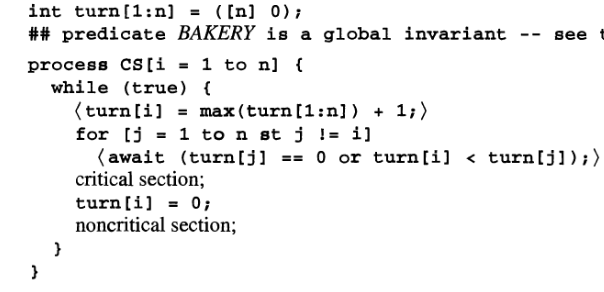
\includegraphics[scale=0.4]{img/bakery.png} \\
L'algoritmo di bakery della figura non può essere implementato direttamente su macchine contemporanee. L'assegnazione a turn[i] richiede il calcolo del massimo di \textit{n} valori, e l'istruzione await fa riferimento a una variabile condivisa (turn[j]) due volte. Queste azioni potrebbero essere implementate atomicamente usando un altro protocollo di sezione critica come l'algoritmo tie-breaker, ma ciò sarebbe abbastanza inefficiente.




\section{Sincronizzazione a barriera}
Forma di sincronizzazione più avanzata che viene utilizzata quando ci sono degli algoritmi in cui i processi devono fare delle cose e prima di passare alle iterazioni successive bisogna aspettare che tutti gli altri abbiano finito.
\paragraph{DEF} Una barriera è un \textbf{punto di sincronizzazione} che tutti i processi devono raggiungere prima che qualsiasi processo sia autorizzato a procedere.

Molti problemi possono essere risolti usando algoritmi iterativi che terminano quando la risposta finale è stata calcolata o - nel caso di molti algoritmi numerici - quando la risposta finale è convergente. Un tale algoritmo tipicamente manipola un array di valori e ad ogni iterazione esegue lo stesso calcolo su tutti gli elementi dell'array.
Quindi, possiamo spesso usare processi multipli per calcolare parti disgiunte della soluzione in parallelo. 
\begin{verbatim}
while (true) {
co [i = 1 to n]
code to implement task i;
oc
}
\end{verbatim} 
Questo approccio è inefficiente perché \textit{n} processi vengono creati e distrutti ad ogni iterazione.
Un'alternativa più efficiente è quella di creare i processi una volta e poi farli sincronizzare alla fine di ogni iterazione.

\subsection{Shared Counter}
\begin{verbatim}
int count = 0;
process Worker[i = 1 to n] {
while (true) {
code to implement task i;
(count = count + 1;)
(await (count == n);)
}
}
\end{verbatim}
Il modo più semplice per specificare i requisiti di una barriera è quello di utilizzare un intero condiviso, \textbf{count}, che inizialmente è zero. Supponiamo che ci siano \textbf{n} processi di lavoro che devono incontrarsi ad una barriera. Quando un processo arriva alla barriera, incrementa il conteggio; quando il conteggio è n, tutti i processi possono procedere. Questa specifica porta al problema dell'azzeramento di count. \textit{count} deve essere resettato a 0 solo dopo che tutti i processi hanno passato la barriera, altrimenti qualcuno resta bloccato; inoltre deve essere resettato prima che qualsiasi processo tenti di incrementarlo di nuovo.
Questo problema può essere risolto utilizzando due variabili contatore, uno
che conta fino a \textit{n} e un altro che conta fino a \textit{0}, con i ruoli dei contatori vengono \textbf{scambiati dopo ogni fase}. Tuttavia, ci sono ulteriori problemi pragmatici con l'uso di contatori condivisi. Primo, devono essere incrementati e/o decrementati come azioni atomiche. Secondo, quando un processo è ritardato, sta esaminando continuamente il conteggio. Nel caso peggiore, n-1 processi potrebbero essere ritardati in attesa che l'ultimo processo arrivi alla barriera. Questo potrebbe portare a grave contesa di memoria (hotspot), tranne che su multiprocessori con cache coerenti. Ma anche allora, il valore del conteggio cambia continuamente, quindi ogni cache deve essere aggiornata. Quindi è appropriato implementare una barriera usando i contatori solo se la macchina di destinazione ha istruzioni di incremento atomico, cache coerenti e un efficiente aggiornamento della cache. Inoltre, n dovrebbe essere relativamente piccolo.

\subsection{Flags and coordinators}
Un modo per evitare il problema della contesa della memoria è quello di distribuire l'implementazione del conteggio utilizzando n variabili che si sommano allo stesso valore. In particolare viene utilizzato un array in cui ognuno segnala che è arrivato in fondo e si evita la contesa della memoria perché l'array conterrà valori grandi tali da essere memorizzati in linee differenti di cache. Ma anche se gli elementi dell'array si trovano in linee differenti di cache, comunque verranno continuamente letti e sommati da tutti i processi, reintroducendo il problema della memoria.

Per risolvere entrambi i problemi di contesa della memoria e di reset si usa un set addizionale di valori condivisi e impiegando un processo addizionale, Coordinatore. Invece di avere ogni processo lavoratore che somma e verifica i valori di arrivo, lasciamo ogni lavoratore aspetti che un singolo valore diventi vero.
In pratica, i \textbf{worker} settano gli elementi dell'array \textbf{arrive} a 1 e aspettano che gli elementi di \textbf{continue} siano settati a 1.
Il \textbf{Coordinatore} aspetta che tutti gli elementi di \textbf{arrive} siano 1, quindi setta gli elementi di \textbf{continue} a 1.
La contesa della memoria non è un problema poiché i processi aspettano che siano settate diverse variabili e queste variabili potrebbero essere memorizzate in diverse linee di cache.
\textit{arrive} e \textit{continue} sono quindi chiamati variabili \textbf{flag}.\\

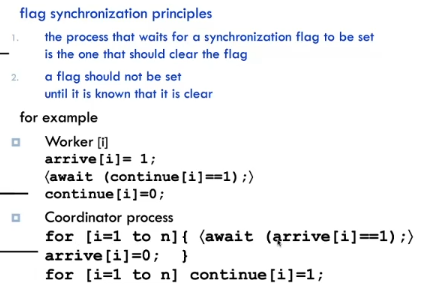
\includegraphics[scale=0.6]{img/flag.png} \\ \\

\paragraph{Problemi}
-richiede un processo extra (processore extra?)\\
-il tempo di esecuzione del coordinatore è proporzionale al numero di lavoratori
\paragraph{Soluzione}
rendere il lavoratore anche un coordinatore, ad es. organizzarli in un albero, cioè i segnali \textit{arrive} vanno su per l'albero e i segnali \textit{continue} vanno verso il basso.\\ \\
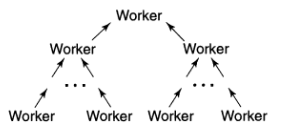
\includegraphics[scale=0.6]{img/tree.png} \\ \\

\subsection{Symmetric barriers}
symmetric n-process barrier is constructed from pairs of simple, two-process barriers.\\ \\ 
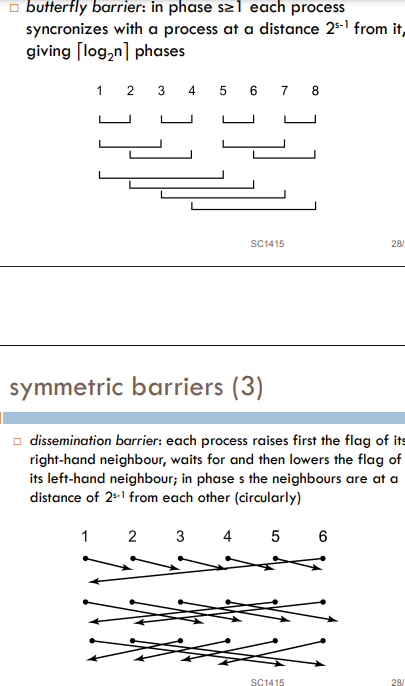
\includegraphics[scale=0.7]{img/butterfly.png} \\ \\

\section{Semafori}
\marginpar{videolezione 2021-10-08}





















\end{document}